\apendice{Plan de Proyecto Software}

\section{Introducción}
Para el correcto desarrollo del proyecto se seguirá una planificación temporal y se desarrollará una planificación económica para ver el coste económico aproximado del producto desarrollado a lo largo del proyecto. Además, se dispondrá de un apartado donde consultar la viabilidad legal del desarrollo del proyecto.

\section{Planificación temporal}
% Inicio de la figura
\begin{figure}[h]
    \centering
    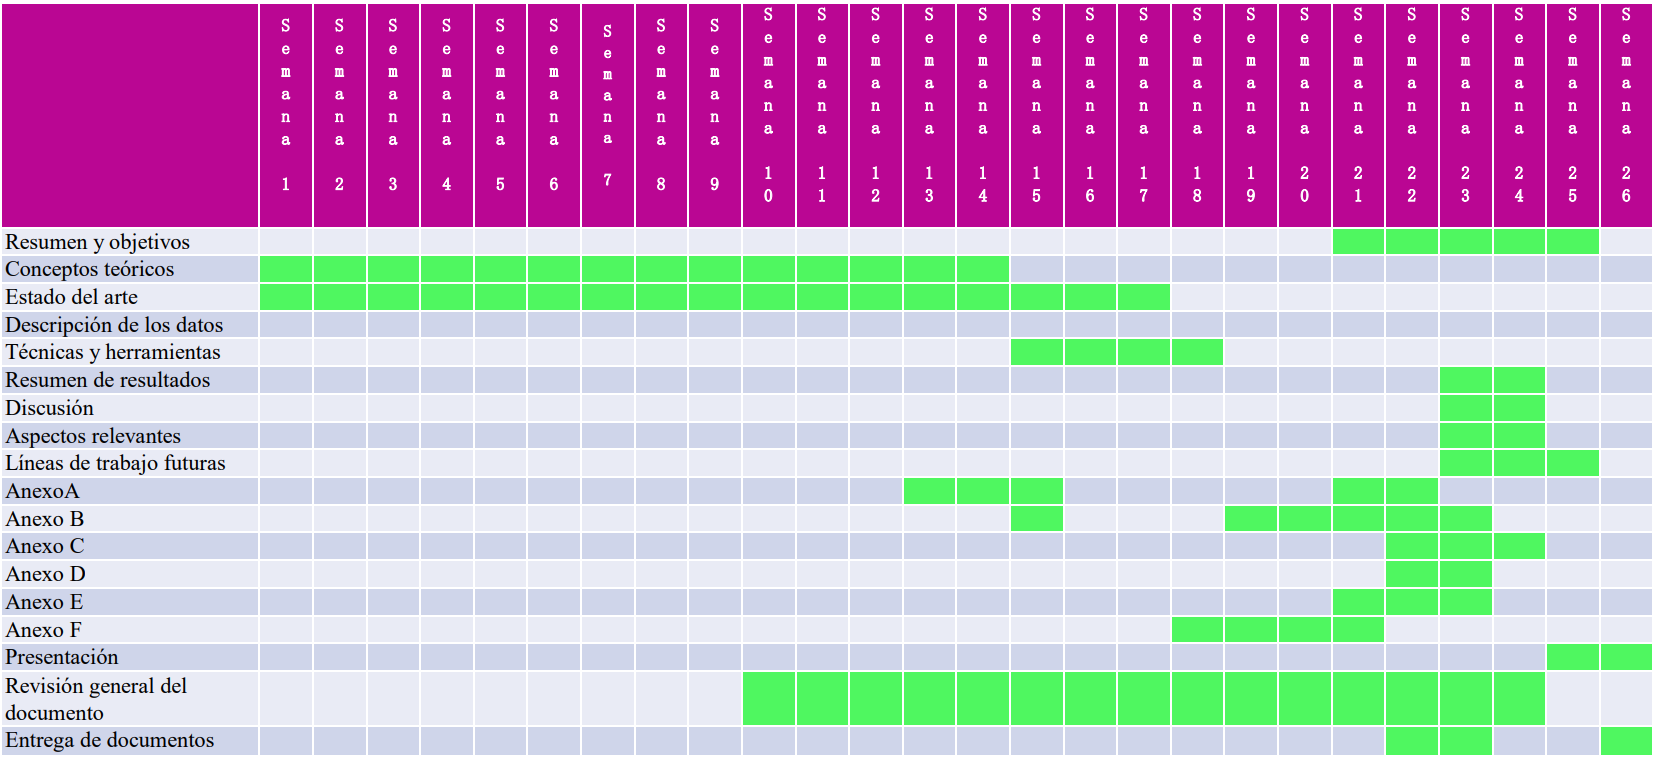
\includegraphics[width=1\textwidth]{img/PlanificacionTemporal.png}
    \caption{Planificación temporal seguida para la realización de este proyecto.  Fuente propia.}
    \label{fig:planTemporal} 
\end{figure}

En la planificación temporal se puede ver cada apartado de la memoria y los anexos desarrollados a lo largo de las semanas. 

\section{Planificación económica}

Para obtener una buena planificación económica se deberán identificar los costes tanto personales como materiales y de desarrollo y los ingresos relacionados con el prototipo.

Los costes personales se calcularán en función del salario medio de un Ingeniero de la Salud durante un periodo aproximado de 6 meses durante media jornada\footnote{La media jornada constará de unas 4 horas al día durante 5 días a la semana, es decir, 20 horas semanales.}, lo que suma unas 540 horas de trabajo totales. Teniendo en cuenta que el sueldo neto medio de un ingeniero con menos de 3 años de experiencia ronda los 1392,8€ al mes a jornada completa \cite{SueldoBruto}, a media jornada cobrará unos 696,4€ al mes. Por lo tanto, los costes de personal se podrían resumir en la siguiente tabla.

% ----------------------------------------------------
% Tabla del desglose económico de costes personales.
\begin{table}[h!]
\centering
\begin{tabular}{ |m{5cm} m{3cm}|  } 
\hline
\cellcolor[HTML]{EFEFEF}\textbf{} & \cellcolor[HTML]{EFEFEF}\textbf{Costes}\\

Sueldo neto mensual           & {696,4€} \\

Sueldo bruto mensual                & {799,79€}\\
\hline
\cellcolor[HTML]{EFEFEF}\textbf{Total en los 6 meses}                & \cellcolor[HTML]{EFEFEF}{4798,74€} \\
\hline
\end{tabular}
\caption{Resumen de costes personales.}
\end{table}

Como primeros gastos relacionados con los equipos de desarrollo, el ordenador que se ha empleado y la licencia de Office que se ha empleado para la realización de algunas partes del proyecto, con una amortización\footnote{La amortización se calcula con la diferencia del coste del equipo y del coste residual a los 4 años (un 40\% del coste del equipo) todo ello divido entre el periodo de amortización, que en este caso serán unos 4 años.} \cite{amortizacion} en unos 4 años. No se incluyen gastos de otros softwares, porque se han empleado herramientas de código abierto y gratuitas.

% ----------------------------------------------------
% Tabla del desglose económico de equipos de desarrollo.
\begin{table}[h!]
\centering
\begin{tabular}{ |m{5cm} m{3cm} m{3cm}|  } 
\hline
\cellcolor[HTML]{EFEFEF}\textbf{} & \cellcolor[HTML]{EFEFEF}\textbf{Costes}& \cellcolor[HTML]{EFEFEF}\textbf{Amortización}\\

Ordenador ASUS           & {700€} & {105€}\\

Office 365 personal anual              & {69€} & {10,35€}\\
\hline
\cellcolor[HTML]{EFEFEF}\textbf{Total en los 6 meses}                & \cellcolor[HTML]{EFEFEF}{769€} & \cellcolor[HTML]{EFEFEF}{115,35€} \\
\hline
\end{tabular}
\caption{Resumen de costes de equipos de desarrollo amortizados en 4 años.}
\end{table}


Para el cálculo del gasto de los materiales del desarrollo del prototipo, se tienen en cuenta los costes de los componentes y los gastos de realización del prototipo, mientras que para obtener los posibles ingresos se tendrá en cuenta el beneficio, gastos imprevistos e I+D del producto, para posibles mejoras en e futuro. La suma de gastos e ingresos nos devolverá el precio final aproximado del dispositivo. No se incluyen los gastos personales, ni de equipos, dado que estos gastos se incluirían en caso de producción del dispositivo final.


% ----------------------------------------------------
% Tabla del desglose económico de las versiones realizadas.
\begin{table}[h!]
\centering
\begin{tabular}{ |m{4cm}|m{4cm}|m{2cm}|m{2cm}|  } 
\hline
\cellcolor[HTML]{B9E3F0}\textbf{} & \cellcolor[HTML]{B9E3F0}\textbf{Cálculos} & \cellcolor[HTML]{B9E3F0}\textbf{Versión 1}& \cellcolor[HTML]{B9E3F0}\textbf{Versión 2}\\

\hline
\cellcolor[HTML]{EFEFEF}\textbf{Gastos de los componentes}             & {Suma de los precios de cada componente del producto}   & 27€ & 32.5€\\
\hline
\cellcolor[HTML]{EFEFEF}\textbf{Gastos de producción}                & {10\% del precio de los componentes} & 2.7€ & 3.25€\\
\hline
\cellcolor[HTML]{EFEFEF}\textbf{Ingresos destinados a beneficio}                & {5\% del total de gastos} & 1.48€ & 1.79€\\
\hline
\cellcolor[HTML]{EFEFEF}\textbf{Gastos imprevistos e I+D} & {10\% del total de gastos} & 2.97€ & 3.58€\\
\hline
\cellcolor[HTML]{EFEFEF}\textbf{Precio Total} & {Suma de los gastos e ingresos} & \textbf{34.15€} & \textbf{41.10€}\\
\hline
\end{tabular}
\caption{Resumen de gastos y precio total del producto}
\end{table}

El prototipo de la versión 1, en la que se emplea el sensor SW520D\cite{SW520D_1}, tiene un coste final aproximado\footnote{La planificación económica será variable en el tiempo y durante el desarrollo del producto, por lo que se trata de precios totales aproximados. Igual para el prototipo versión 2.} de unos 34.15€, precio que podría ser menor al crear nuestro propio microcontrolador o utilizar una alternativa similar a Arduino, puesto que es el elemento que más aumenta el precio de la solución, siendo el precio del resto de los componentes aproximadamente unos 3€.

Por el contrario el prototipo de la versión 2, en el que se emplea el módulo MPU-6050\cite{MPU6050_1,MPU6050_2}, tiene un coste final aproximado de unos 41.10€, precio que también podría disminuir al crear nuestro propio microcontrolador o utilizar una alternativa a Arduino, ya que sin el microcontrolador Arduino el precio ronda los 8.5€.


\subsection{Desglose de los precios de los componentes del prototipo Versión 1}

Se han tenido en cuenta los precios más bajos encontrados de cada componente necesario. Estos precios incluyen el porcentaje de IVA y se han calculado en base a los precios del proveedor Amazon España\cite{amazon}.
\begin{itemize}
    \item Arduino UNO R3: 24€
    \item Resistencias (330 \textOmega, 2x220 \textOmega, 33 \textOmega, 1000 \textOmega): 0.05€
    \item Zumbador pasivo: 0.25€
    \item Motor de vibración: 1€
    \item Transistor: 0.05€
    \item SW520D: 0.5€
    \item Led azul: 0.02€
    \item Pulsador: 0.05€
    \item Otros elementos variados: 1€
    
\end{itemize}

\subsection{Desglose de los precios de los componentes del prototipo Versión 2}
Se han tenido en cuenta los precios más bajos encontrados de cada componente necesario. Estos precios incluyen el porcentaje de IVA y se han calculado en base a los precios del proveedor Amazon España\cite{amazon}.
\begin{itemize}
    \item Arduino UNO R3: 24€
    \item Resistencias (2x330 \textOmega, 2x220 \textOmega, 33 \textOmega, 1000 \textOmega): 0.06€
    \item Zumbador pasivo: 0.25€
    \item Motor de vibración: 1€
    \item Transistor NPN: 0.05€
    \item MPU-6050: 6€
    \item Led azul: 0.02€
    \item 2x Pulsador: 0.10€
    \item Otros elementos variados: 1€
    
\end{itemize}


\section{Viabilidad legal}

Se debe tener en cuenta en todo momento que el dispositivo sea completamente seguro y no afecte negativamente al usuario. Para ello, existen legislaciones específicas a cada fase del desarrollo y comercialización del producto que se deben cumplir para obtener un dispositivo seguro y regulado.

Se pueden diferenciar 3 fases, una primera fase de creación de la idea, diseño y desarrollo y realización de pruebas, una segunda fase de comercialización y la última fase de posventa, donde se incluyen las demandas y la gestión de los datos de los usuarios.

Durante la primera fase de creación de la idea, diseño y desarrollo del producto y realización de pruebas, todos los movimientos que se realicen se deberán ajustar a las siguientes legislaciones:
\begin{itemize}
    \item Ley 24/2015\cite{patentes}, Ley de Patentes, dónde se regula todo lo relacionado con la protección de invenciones empleando patentes, desde el registro de las patentes, invenciones patentables, el derecho a la patente y los procedimientos para pedir una patente.
    % Referencia: 
    % https://www.boe.es/buscar/act.php?id=BOE-A-2015-8328
    
    \item Real Decreto Legislativo 1/1996\cite{PropIntelectual} relativo Ley de Propiedad Intelectual que regulariza la protección del derecho de autor y de derechos similares.
    % referencia:
    % https://boe.es/buscar/act.php?id=BOE-A-1996-8930
    
    \item Los productos sanitarios se rigen por la Agencia española de medicamentos y productos sanitarios (AEMPS)\cite{AEMPS}. En este proyecto nos interesan especialmente el Real Decreto 1591/2009\cite{prodSanitario1} que regula todo lo relativo a los productos sanitarios, desde su desarrollo a su venta, y el Real Decreto 437/2002\cite{prodSanitario2} establece las pautas para la concesión de licencias de fabricación y desarrollo de productos sanitarios.
    % Referencias:
    % https://www.aemps.gob.es/productos-sanitarios/legislacion-sobre-productos-sanitarios/
    % https://www.boe.es/buscar/doc.php?id=BOE-A-2009-17606
    % https://www.boe.es/buscar/doc.php?id=BOE-A-2002-10228
    
    \item Reglamento de la UE 2017/745\cite{ProdSanitariosEU} de Productos Sanitarios de la Unión Europea este reglamento establece requisitos y regula la comercialización de productos sanitarios en la Unión Europea, con el fin de garantizar un dispositivo de calidad, eficaz y completamente seguro.
    % Referencia:
    % https://eur-lex.europa.eu/legal-content/ES/TXT/?uri=uriserv:OJ.L_.2017.117.01.0001.01.SPA&toc=OJ:L:2017:117:TOC
    
    \item Además, durante todo el desarrollo del producto se deberá cumplir con la normativa laboral española\cite{normaLaboral}, que incluye leyes y reglamentos como pueden ser el Estatuto de los Trabajadores, la Ley de Prevención de Riesgos Laborales o la Ley de Igualdad.
    % Referencia
    % https://www.boe.es/biblioteca_juridica/codigos/codigo.php?id=93&modo=2&nota=0&tab=2
    
\end{itemize}

Si se consigue crear el dispositivo en base a todas las leyes anteriores y se quisiera sacar a mercado se deberán cumplir también con los siguientes requisitos legales:
\begin{itemize}
    \item La Ley 34/2002\cite{comercioElectronico} de Servicios de la Sociedad de la Información y de Comercio Electrónico, en caso de que se realice una tienda web oficial de comercialización del dispositivo.
    % Referencia:
    % https://www.boe.es/buscar/act.php?id=BOE-A-2002-13758
    
    \item Además, se deberán tener en cuenta otras leyes\cite{comercio} como la Ley 7/1996\cite{comercioMinorista} de Ordenación del Comercio Minorista.
    % Referencia:
    % https://www.boe.es/buscar/act.php?id=BOE-A-1996-1072
    % https://www.boe.es/biblioteca_juridica/codigos/codigo.php?id=35&modo=2&nota=0&tab=2
\end{itemize}

Por último, si el dispositivo se ha puesto a la venta se debe pensar en los requisitos legales que se necesitarán cumplir a partir del momento de la primera venta. Alguno de estos requisitos serán:
\begin{itemize}
    \item Ley Orgánica 3/2018\cite{protDatos} de Protección de Datos Personales y garantía de los derechos digitales. Para poder proteger cualquier información que identifique a una persona, de forma confidencial. Además, el usuario debe estar correctamente informado del tratamiento de sus datos, además el acceso al tratamiento de sus datos debe ser claro y accesible.

    El usuario tendrá derecho al acceso de sus datos, derecho de rectificación y supresión de sus datos, derecho a la limitación del tratamiento de sus datos, derecho a la portabilidad de sus datos y el derecho a oponerse al tratamiento de sus datos. Por todo ello el tratamiento de sus datos debe ser tras la confirmación clara del consentimiento informado del tratamiento de sus datos.
    % Referencia:
    % https://www.boe.es/buscar/doc.php?id=BOE-A-2018-16673

    \item Reglamento UE 2016/679\cite{protDatosEU} relativo a Protección de las Personas Físicas en lo que respecta al tratamiento de datos personales y circulación de estos Datos. Donde se define que se debe garantizar la protección de los datos con los que se trabaja, además de notificar brechas de seguridad o exposición de datos al usuario.
    % Referencia:
    % https://eur-lex.europa.eu/ES/legal-content/summary/general-data-protection-regulation-gdpr.html
\end{itemize}

Además el dispositivo deberá contar con un certificado CE\cite{certificadoEuropeo}, que garantizará que el dispositivo cumple con los requisitos de seguridad, protección y sanidad europeos. Una vez se obtenga el certificado el dispositivo podrá ser comercializado legalmente en la Unión Europea.
% Referencia:
% https://europa.eu/youreurope/business/product-requirements/labels-markings/ce-marking/index_es.htm